\chapter{The Graal Compiler Infrastructure} \label{chp:graal}
Graal is a new approach to Java compiler engineering. Here, Graal is introduced and technically assessed. It's strengths and weaknesses are also evaluated.

\section{Background} \label{sec:graal/background}
The basis of the project is the Graal compiler infrastructure \citep{Graal}. Graal is an experimental project developed mainly at Oracle Labs (although there are some additional collaborators at AMD) under the OpenJDK programme.
	
The aim of the Graal project is to develop a Java compiler written in Java itself - `\textit{a quest for the JVM to leverage its own J}'. Graal is, in essence, a Java compiler written in Java. However, this doesn't fully explain the Graal project.
	
Virtually all languages used commonly in industry have had their compilers go through a so-called `bootstrap' process. This bootstrapping process involves writing the compiler for a language in the language it is intended to compile. In many cases the first version of a compiler is written in a different language - commonly used languages include the standard C and C++ due to their performance. There are many examples of this in the real-world - GCC is written in a combination of C and C++\footnote{Although the project is currently converting all C code to C++}, LLVM/Clang is written in C++ etc. There are several advantages to this approach - in essence, this process is a kind of informal proof that the language has matured to a level that is capable of supporting a program as complicated as a compiler. In effect, bootstrapping a compiler displays shows that a language (and associated platform) has a certain level of `maturity'; that it is now ready for large software projects (or at least not totally unprepared for them).

Graal is an attempt to bring this approach to the Java Virtual Machine. Note that there are other projects with attempts to bootstrap parts of the Java platform - for example, the Maxine VM is a Java virtual machine written in Java. However, because Java is unlike most other platforms (in that it not only requires a compiler, but also a virtual machine, class library and such), the compiler has, until the advent of the Graal project, remained written in C++.

Another feature of Graal is that it allows users (of the compiler) to interface directly with the compiler. Common compilers (GCC, ICC etc) are seen as `black-boxes', where a user invokes the compiler, waits for a while, and then a resulting object file or binary is produced. Graal is a part of a new generation of compilers that expose APIs to users, which means users can change parts of the compilation process to suit their needs, ease debugging and other such advantages. With modern languages and platforms being required to target multiple different machine classes (module, desktop, laptop and server/cloud), this is a crucial advantage over more conventional languages and platforms. There are only a few examples of this new generation of compiler, but another - somewhat more mainstream example - is Microsoft's Rosyln project \citep{RoslynProject} for their .NET platform. The new Windows Runtime include deep metadata integration into the platform (which is the basis for, amongst other things, the Common Object System in .NET languages\footnote{Which allows inter-language types to be considered equivalent - a C int is semantically equivalent to a C++ int, a C\# int, a JavaScript int and so on}).

\begin{figure}
	\centering
	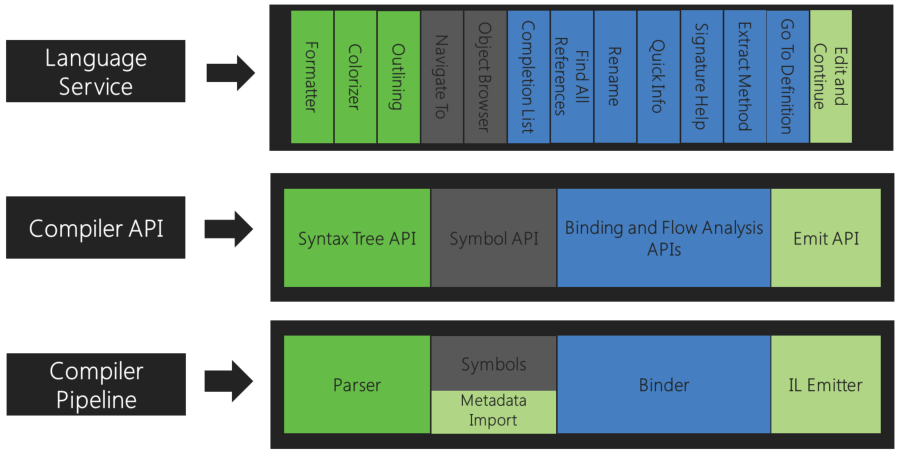
\includegraphics[width=0.7\textwidth]{graphics/roslyn-pipeline.pdf}
	\label{fig:roslyn-pipeline}
	\caption{The compiler pipeline in Microsoft Roslyn, a similar project to Graal. Roslyn operates at a higher level than Graal, instead manipulating abstract syntax trees. [Figure \citealp{RoslynProject}]}
\end{figure}

\section{Introduction} \label{sec:graal/introduction}
Graal is somewhat different than other compilers. As opposed to other compilers, which use a combination of parsers and lexers to produce their IRs from source code, Graal builds the IR from Java bytecode instead. This approach has several advantages for this project, the main being that we cannot assume that the source code is available to many legacy programs. Another advantage to this approach is that it would allow the detection mechanism to not only be performed upon user-provided programs, but also system-level libraries as well (for example, the Java Collections Framework). Lastly, it would allow the instrumentation of all JVM languages, not just Java. There are many languages which have been designed for the JVM, such as Scala, Groovy and Clojure, and there are also some languages which have been ported to the JVM such as Python (through Jython), Ruby (through JRuby) and PHP (through Quercus).

\section{Intermediate Representations} \label{sec:graal/ir}
Like many compilers, Graal uses several different internal representations at different stages of compilation. Each of the representations has a distinct, non-overlapping use case; despite this the graphs are somewhat similar in structure.

As is common in many compilers, Graal uses graphs for intermediate representations. These graphs combine several different kinds of graph together into a single form, such as control flow and memory dependency (data flow).

To illustrate this, consider the figure \ref{fig:vector-inline}, created using the Ideal Graph Visualiser (\textit{IGV}).

\begin{figure}
	\centering
	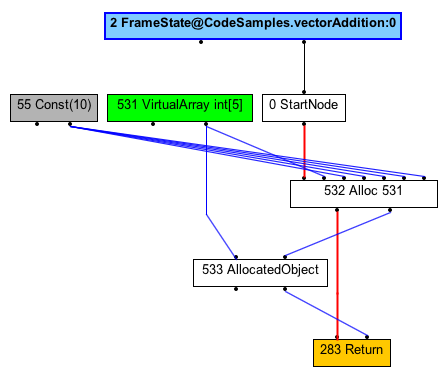
\includegraphics[width=0.7\textwidth]{graphics/loop-inline.png}
	\caption{Graal HIR created for a vector addition using two array literals}
	\label{fig:vector-inline}
\end{figure}

The format for graph visualisations is the following:
\begin{itemize}
	\item Red edges represent control flow
	\item Blue edges represent memory dependence
	\item Black edges are defined as edges which are not control flow or memory dependence. In reality, they are mainly used for associating \texttt{FrameState} nodes where appropriate
\end{itemize}

The text inside nodes uses the following format:

\texttt{<node-id> NodeName <additional>}

In some cases, \texttt{<additional>} contains the value associated with the code (for subtypes of \texttt{ValueNode}). Node IDs are unrelated to the ordering within the graph. Time is represented on the y-axis of the graph, flowing down the page (so in the case of figure \ref{fig:vector-inline}, node 0 (\texttt{StartNode}) is executed first, followed by node 532 and 283 in that sequence).

\autoref{fig:vector-inline} is a representation of a vector addition using two \texttt{int} array literals as arguments. The original source code contains a loop, which itself contains two array load operations, an addition and an array store operation. From it, we can see clearly the different kinds of node relationships in Graal's IR. The \texttt{StartNode} is the start of the method, which is followed by an allocation (notice that the loop was been optimized away by Graal), the result of which is then returned from the method.

The allocate has two actual memory dependencies:

\begin{itemize}
	\item A \texttt{VirtualArray} node is used to create an array. We can see that the type of this array is \texttt{int[]} with length five.
	
	\item A \texttt{ConstantNode} is referenced five times, one for each position of the array.
\end{itemize}

Without both of these dependencies, the compiler cannot create the array, and assign the correct values. Note that, because the JVM allocates default values of zero to declared-yet-unassigned variables, if the \texttt{ConstantNode} was not used, the array would consist of zeros.

\section{Graph Transformations} \label{sec:graal/transformations}
One of the ways the abilities of Graal are manifested is through it's capacity to apply transformations to the various intermediate representations. The main use for this is to allow users of the compiler to add custom behaviour at the various stages of the compilation process, but the mechanism extends to additional uses. For example, custom behaviour can be inserted into programs, as well as the graphs dumped for inspection in external tools.

As of the time of writing, Graal uses a hybrid approach to transforming graphs between the IRs - suites and phases. They are, in effect, essentially the same thing - they both consist of a sequence of transformations (in Graal terminology, a \textit{phase}) which are applied to a graph in a well-defined order (although the user can change the ordering if required, as well as disable certain phases\footnote{A common usage for this is to disable the inlining optimisation.}. The result of a sequence of phases is the representation used at the next lower-level of abstraction. The three phases in Graal are high-level, mid-level, and low-level.

{\small \textit{Todo: clear up the difference between runtime-specific lowering and target-specific lowering.}}

The high-level phase is used mainly for the graph-building phase. Graal uses the concept of \texttt{ResolvedJavaMethod}s, which are internal `linkages' to constant pools found within \texttt{.class} files. It is also used for runtime-specific lowering\footnote{\emph{Lowering} is a mechanism to convert a complex bytecode into a simpler one, much like the difference between RISC and CISC architectures}, for example to handle multiple machine instruction set architectures - although the Java language is unconcerned with JVM implementation details such as the endianness of the machine's CPU, the runtime must, by definition, be aware of this fact. Examples of runtime-specific lowering are found throughout Graal, but examples include multiple implementations of the \texttt{GraalRuntime} interface - one for each ISA that Graal supports. Single Static Assignment (SSA) form is used at the high-level in order to allow for optimisations to be performed.

Mid-level phases remove the SSA form, and includes target-specific lowering. The low-level phases are analogous to the backends of more traditional compilers, and deals with low-level issues such as register allocation and code generation.

It is important to note that lowering is an iterative process, because a given lowering phase may result in further `lowerable' nodes being added to the graph.

There are two main classes of lowering in Graal, and they are split into nodes which implement \texttt{Lowerable} and those which implement \texttt{LIRLowerable}. \texttt{Lowerable} nodes are transformed between the high-level and mid-level, and \texttt{LIRLowerable} nodes are transformed between the mid-level and low-level -- figure \ref{fig:lowering-stages} shows this diagrammatically.

\begin{figure}
	\centering
	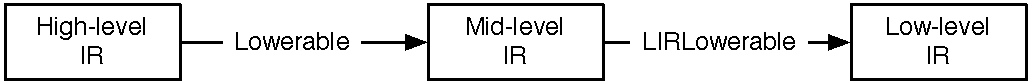
\includegraphics[width=1.0\textwidth]{graphics/lowering-stages.pdf}
	\caption{Relationships between IR levels and lowering types in Graal}
	\label{fig:lowering-stages}
\end{figure}

	\subsection{The \texttt{.class} File Format - Constant Pools} \label{sec:graal/classformat}
	In order to properly understand \texttt{ResolvedJavaMethod}s, one needs to understand some parts of the \texttt{.class} file format. The source for this section is the Java Virtual Machine specification \citep[p.~69]{JVMSpec}.
		
	\texttt{.class} files are structured containers for Java bytecode streams. However, they are not `plain old data structures', as would be indicated by that description. Instead, they are laid out in such a way to increase performance for the JVM.
				
	Unlike some other executable file formats, the JVM does not rely on the (relative) positions of the various kinds of definition permitted. In this context, constants refer to \emph{all} immutable identifiers - and not simply to the language-level construct of constants (\eg, \texttt{public static final int THOMAS\_KLAUS = 9;}). Each constant has an entry in the \emph{constant pool} - a table containing \texttt{cp\_info} structures. A \texttt{ResolvedJavaMethod} contains a link to the offset of a \texttt{cp\_info} structure for a method.
		
\section{Snippets} \label{sec:graal/snippets}
In order to engineer the lowering and optimisations mechanisms in a way that follows `good'\footnote{For some definition of `good'} manner that follows solid software engineering principles (low code reproduction, cohesion and linkage \etc), Graal uses the snippets mechanism.

Snippets are Graal graphs represented as Java source methods. They are used for lowering bytecodes with runtime-dependent semantics, such as \texttt{CHECKCAST}\footnote{\url{http://homepages.inf.ed.ac.uk/kwxm/JVM/checkcast.html}}. Snippets allow certain complex bytecodes to be replaced with simpler ones. Furthermore, snippets have the additional constraint that they must be deoptimisation (see section \ref{sec:graal/deopt}) free.

Each class of snippets has an associated template, which provides the mechanism through which snippets are instantiated, and the graph modified. These are usually made available through a static nested class of the snippet class. Every time a snippet is activated, the template class creates a template for the snippet, adds arguments (via the \texttt{Arguments} class), and then modifies the graph, replacing the target bytecodes with the snippet.

Snippets are highly related to lowering, as they are used to lower nodes between the different IRs. 
	
\section{Replacements} \label{sec:graal/replacements}
In this feature, which is perhaps unique amongst compiler implementations, Graal allows the user to dynamically change implementations of methods at compile-time -- in other words, Graal allows compile time method polymorphism. In a sense, replacements are similar to snippets (section \ref{sec:graal/snippets}), in that they both represent graph replacements. They differ in that snippets are a low-level abstraction, used for replacing bytecodes with other bytecodes, whereas replacements are for replacing method implementations.

The idea is simple: to replace the body of a method dynamically, at compile-time. This requires performing a compilation on both the replacer and replacee. The name and signatures of the methods must be identical.

This mechanism is exposed via both the \texttt{Replacements} interface, and the\\ \texttt{{@}MethodSubstitution} annotation. This annotation includes various metadata, such as whether the replaced method should be substituted in all cases, and the identifier and signature of the method that will be replaced. The class which this is defined is then passed to an implementation of the \texttt{Replacements} interface, which performs a runtime-appropriate transformation.

In all cases, however, the basic idea of the transformation is the same. Both methods are compiled, and the surrounding pre-call and post-return of the replacee\footnote{Of course, at this stage this compilation should have \emph{already} been performed}. The nodes for the method starts and returns (or end nodes) are replaced until the transformation is complete. Figure \ref{fig:method-subs} displays this mechanism.

\begin{figure}
	\centering
	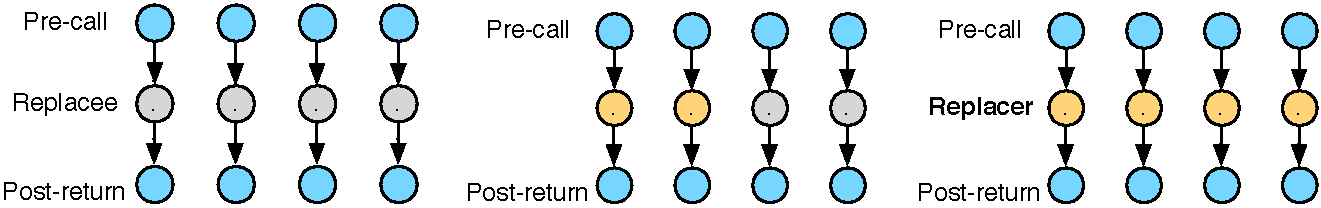
\includegraphics[width=\textwidth]{graphics/graph-replacement.pdf}
	\caption{Method substitution in Graal}
	\label{fig:method-subs}
\end{figure}

\section{Optimisations and Deoptimisations} \label{sec:graal/deopt}
For maximum performance, Graal applies optimisations aggressively and speculatively. The potential performance advantages of speculative optimisation outweighs the possible downside of occasionally requiring deoptimisation. In addition, probability of certain blocks being executed can be computed at compile-time, which in-essence provides Graal with additional metadata regarding which blocks it may prove fruitful to optimise. If a loop is to be executed 100 times, with a low probability of exception-causing errors being thrown per iteration, it makes sense to optimise the loop for the cases where no exception will be thrown. The performance advantage of doing so will be greater than the performance decrease as a result of deoptimisation in the few(er) cases where it will be required.

Some of the optimisations that Graal applies are described here.

\begin{itemize}
	\item \textbf{Dead and unreachable code elimination}
		
		Dead code is code that may be executed, but has no effect on program correctness or semantics (\ie, it has no meaning \citep[p.~533]{DragonBook}). Code is said to be unreachable if there are no possible inputs which would result in execution of the block the statements exist in.
	
	\item \textbf{Type-checked method inlining}
	
		Method inlining (also called \textit{procedure integration}) replaces calls to procedures with copies of their bodies \citep[p.~465]{ACDI}. However, in some cases the result of these transformations may not be type-safe, even in statically-typed languages such as Java \citep{Magnusson2002}. However, transformations are possible that ensure these method inlings are type-safe.
	
	\item \textbf{Probability of exception throwing}
		
		Many nodes in Graal have an associated \emph{probability} - \ie, the probability of their execution, and hence, the basic block within which they lie.
		
		To illustrate, imagine the following loop:
		
		\begin{verbatim}
		for (int i = 1 to 100) {
		    if (i == 100)
		        doSomethingStrange();
		    else
		        doSomethingNormal();
		}\end{verbatim}
		
		In 99\% of cases, \texttt{doSomethingNormal()} will be executed, and in 1\% of cases \texttt{doSomethingStrange()} will be executed.
		
		This behaviour can be used to speculatively merge blocks into \textit{extended basic blocks} - a maximal sequence of instructions beginning with a leader that contains no join nodes other than its first node \citep[p.~175]{ACDI}. These extended basic blocks can then be optimised in the same way that `normal' blocks can be.
		
		If the above example were used, it could optimise for the \texttt{doSomethingNormal()} calls, and use a deoptimisation for the call to \texttt{doSomethingStrange()}.
		
		Probabilities are computed by post-order graph traversal. When it encounters control flow nodes, Graal uses information about the split to divide probability between probability between the successors. At merge nodes, Graal sums the probability of all predecessors. Lastly, loop frequencies are propagated and each fixed node within loops have their probabilities multiplied by the loop's frequency.
		
		{\small\textit{Note}: Graal also includes references to `\texttt{UseExceptionProbabilityForOperations}', but this feature has not yet been completed.}
	
	\item \textbf{Loop limit checks}
	
		This refers to the practice of ``inserting a predicate on the entry path of a loop and raising a common trap if the check or condition fails'' \citep{LoopPrediction}. Loops are split from a single block into several blocks containing a pre-, main and post- loop.
		
		The advantages of approaches based around this technique are three-fold:
		
		\begin{itemize}
			\item Loop predication can be applied to outer loops without code size increment
			
			\item Checks can be eliminated from the entire iteration space
			
			\item The approaches can be applied to loops with calls
		\end{itemize}
\end{itemize}

\begin{figure}
	\centering
	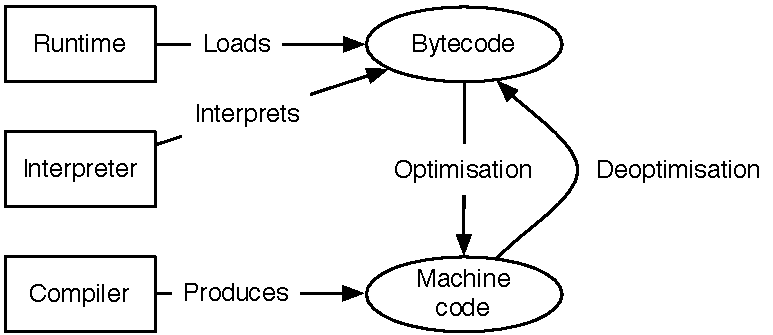
\includegraphics[width=0.8\textwidth]{graphics/jvminternals.pdf}
	\caption{Relationship between optimisations and deoptimisations [adapted from \citealp[p.~24]{Schwaighofer2009}]}
	\label{fig:jvm-internals}
\end{figure}

However, there are some cases where an optimisation has been applied, but it leaves programs in an inconsistent state. In this case, a deoptimisation occurs. More specifically, deoptimisation \citep{Holzle1992} is the process of converting an optimised stack frame into an unoptimised one. In HotSpot, an optimised frame is the result of the JIT compiler and unoptimised frames run using the interpreter. Figure \ref{fig:jvm-internals} shows the interplay between the optimisations and deoptimisations. Optimisation-deoptimisation is controlled through an assumption mechanism - in order to be (or remain) optimised, a set of assumptions must remain true. If any of the assumptions becomes false, the optimisation is broken and deoptimiastion occurs. When deoptimisation occurs, the runtime returns to the bytecode index associated with the optimisation, and executes using the interpreter instead. This technique is used because Graal currently relies on the deoptimisaton framework in HotSpot\texttrademark, which uses the approach described here. 

Deoptimisations can occur for several reasons:

\begin{itemize}
	\item \textbf{Exceptions}: certain kinds of exceptions can trigger deoptimisations as they disrupt control flow. These exceptions are \texttt{NullCheckException}, \texttt{BoundsCheckException}, \texttt{ClassCastException}, \texttt{ArrayStoreException} and \texttt{ArithmeticException}. Additionally, if an exception handler has not been compiled, a deoptimisation will occur.
	
	\item \textbf{Violated assumptions}: if any of the assumptions made during optimisation are violated (\ie, their state is modified), the optimisation is marked as invalidated.
	
	\item \textbf{Unreached code}: if there is unreached code that could not be determined statically, this code is not optimised.
\end{itemize}

\section{Summary} \label{sec:graal/summary}
In this section, we have introduced the Graal compiler infrastructure and some of the advantages that it brings other more traditional compilers. Graal is at the forefront of compiler technology, and is part of a new generation of compilers that provide user-facing APIs. Graal also optimises speculatively and aggressively through a deoptimisation-based model; some of the optimisations and possible reasons for deoptimisations have been introduced.

Graal is distinguished from other compilers by it's flexibility. It is designed to allow users to use the compiler-as-a-service, a new paradigm in compiler technology. Compliers-as-a-service promise a new level of abstraction for compiler technology, with use cases such as code analysis, online refactoring and code generation. Until now, compilers have been a black box which users have little say over the internal workings of. In the future, this will be no longer the case - compilers will adapt to suit the users and programs requirements, and Graal is the first step in this area for the Java world.